% Generated by Sphinx.
\def\sphinxdocclass{report}
\documentclass[a4paper,10pt,english]{sphinxmanual}
\usepackage[utf8]{inputenc}
\DeclareUnicodeCharacter{00A0}{\nobreakspace}
\usepackage{cmap}
\usepackage[T1]{fontenc}
\usepackage{babel}
\usepackage{times}
\usepackage[Bjarne]{fncychap}
\usepackage{longtable}
\usepackage{sphinx}
\usepackage{multirow}

\addto\captionsenglish{\renewcommand{\figurename}{Fig. }}
\addto\captionsenglish{\renewcommand{\tablename}{Table }}
\floatname{literal-block}{Listing }



\title{EQcorrscan Documentation}
\date{April 23, 2015}
\release{0.0.5}
\author{Calum John Chamberlain}
\newcommand{\sphinxlogo}{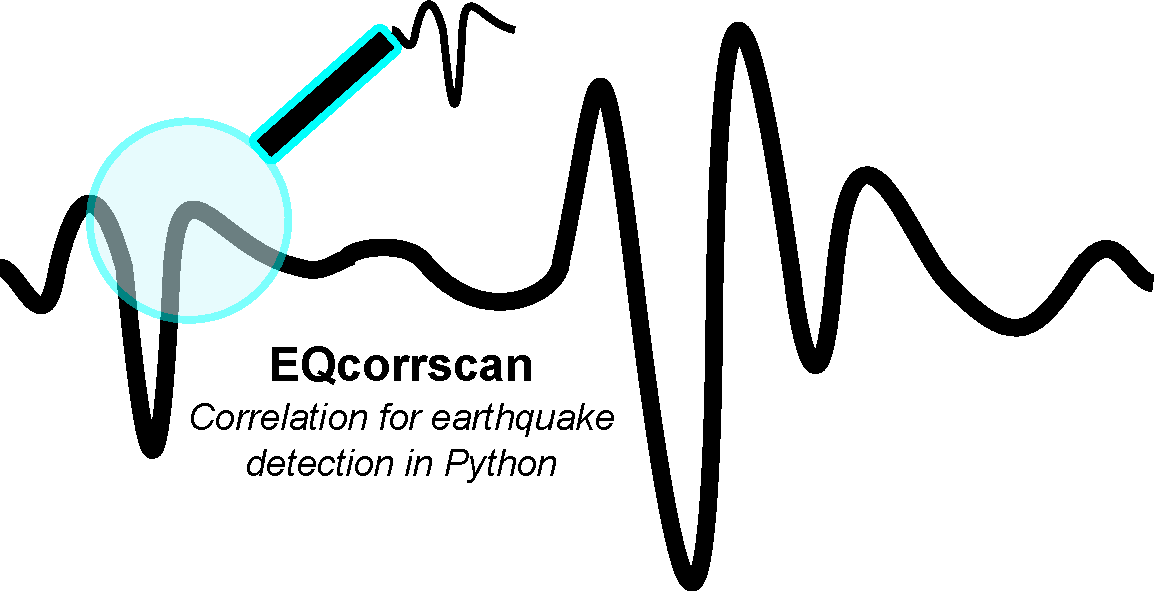
\includegraphics{EQcorrscan_logo.pdf}\par}
\renewcommand{\releasename}{Release}
\makeindex

\makeatletter
\def\PYG@reset{\let\PYG@it=\relax \let\PYG@bf=\relax%
    \let\PYG@ul=\relax \let\PYG@tc=\relax%
    \let\PYG@bc=\relax \let\PYG@ff=\relax}
\def\PYG@tok#1{\csname PYG@tok@#1\endcsname}
\def\PYG@toks#1+{\ifx\relax#1\empty\else%
    \PYG@tok{#1}\expandafter\PYG@toks\fi}
\def\PYG@do#1{\PYG@bc{\PYG@tc{\PYG@ul{%
    \PYG@it{\PYG@bf{\PYG@ff{#1}}}}}}}
\def\PYG#1#2{\PYG@reset\PYG@toks#1+\relax+\PYG@do{#2}}

\expandafter\def\csname PYG@tok@gd\endcsname{\def\PYG@tc##1{\textcolor[rgb]{0.63,0.00,0.00}{##1}}}
\expandafter\def\csname PYG@tok@gu\endcsname{\let\PYG@bf=\textbf\def\PYG@tc##1{\textcolor[rgb]{0.50,0.00,0.50}{##1}}}
\expandafter\def\csname PYG@tok@gt\endcsname{\def\PYG@tc##1{\textcolor[rgb]{0.00,0.27,0.87}{##1}}}
\expandafter\def\csname PYG@tok@gs\endcsname{\let\PYG@bf=\textbf}
\expandafter\def\csname PYG@tok@gr\endcsname{\def\PYG@tc##1{\textcolor[rgb]{1.00,0.00,0.00}{##1}}}
\expandafter\def\csname PYG@tok@cm\endcsname{\let\PYG@it=\textit\def\PYG@tc##1{\textcolor[rgb]{0.25,0.50,0.56}{##1}}}
\expandafter\def\csname PYG@tok@vg\endcsname{\def\PYG@tc##1{\textcolor[rgb]{0.73,0.38,0.84}{##1}}}
\expandafter\def\csname PYG@tok@m\endcsname{\def\PYG@tc##1{\textcolor[rgb]{0.13,0.50,0.31}{##1}}}
\expandafter\def\csname PYG@tok@mh\endcsname{\def\PYG@tc##1{\textcolor[rgb]{0.13,0.50,0.31}{##1}}}
\expandafter\def\csname PYG@tok@cs\endcsname{\def\PYG@tc##1{\textcolor[rgb]{0.25,0.50,0.56}{##1}}\def\PYG@bc##1{\setlength{\fboxsep}{0pt}\colorbox[rgb]{1.00,0.94,0.94}{\strut ##1}}}
\expandafter\def\csname PYG@tok@ge\endcsname{\let\PYG@it=\textit}
\expandafter\def\csname PYG@tok@vc\endcsname{\def\PYG@tc##1{\textcolor[rgb]{0.73,0.38,0.84}{##1}}}
\expandafter\def\csname PYG@tok@il\endcsname{\def\PYG@tc##1{\textcolor[rgb]{0.13,0.50,0.31}{##1}}}
\expandafter\def\csname PYG@tok@go\endcsname{\def\PYG@tc##1{\textcolor[rgb]{0.20,0.20,0.20}{##1}}}
\expandafter\def\csname PYG@tok@cp\endcsname{\def\PYG@tc##1{\textcolor[rgb]{0.00,0.44,0.13}{##1}}}
\expandafter\def\csname PYG@tok@gi\endcsname{\def\PYG@tc##1{\textcolor[rgb]{0.00,0.63,0.00}{##1}}}
\expandafter\def\csname PYG@tok@gh\endcsname{\let\PYG@bf=\textbf\def\PYG@tc##1{\textcolor[rgb]{0.00,0.00,0.50}{##1}}}
\expandafter\def\csname PYG@tok@ni\endcsname{\let\PYG@bf=\textbf\def\PYG@tc##1{\textcolor[rgb]{0.84,0.33,0.22}{##1}}}
\expandafter\def\csname PYG@tok@nl\endcsname{\let\PYG@bf=\textbf\def\PYG@tc##1{\textcolor[rgb]{0.00,0.13,0.44}{##1}}}
\expandafter\def\csname PYG@tok@nn\endcsname{\let\PYG@bf=\textbf\def\PYG@tc##1{\textcolor[rgb]{0.05,0.52,0.71}{##1}}}
\expandafter\def\csname PYG@tok@no\endcsname{\def\PYG@tc##1{\textcolor[rgb]{0.38,0.68,0.84}{##1}}}
\expandafter\def\csname PYG@tok@na\endcsname{\def\PYG@tc##1{\textcolor[rgb]{0.25,0.44,0.63}{##1}}}
\expandafter\def\csname PYG@tok@nb\endcsname{\def\PYG@tc##1{\textcolor[rgb]{0.00,0.44,0.13}{##1}}}
\expandafter\def\csname PYG@tok@nc\endcsname{\let\PYG@bf=\textbf\def\PYG@tc##1{\textcolor[rgb]{0.05,0.52,0.71}{##1}}}
\expandafter\def\csname PYG@tok@nd\endcsname{\let\PYG@bf=\textbf\def\PYG@tc##1{\textcolor[rgb]{0.33,0.33,0.33}{##1}}}
\expandafter\def\csname PYG@tok@ne\endcsname{\def\PYG@tc##1{\textcolor[rgb]{0.00,0.44,0.13}{##1}}}
\expandafter\def\csname PYG@tok@nf\endcsname{\def\PYG@tc##1{\textcolor[rgb]{0.02,0.16,0.49}{##1}}}
\expandafter\def\csname PYG@tok@si\endcsname{\let\PYG@it=\textit\def\PYG@tc##1{\textcolor[rgb]{0.44,0.63,0.82}{##1}}}
\expandafter\def\csname PYG@tok@s2\endcsname{\def\PYG@tc##1{\textcolor[rgb]{0.25,0.44,0.63}{##1}}}
\expandafter\def\csname PYG@tok@vi\endcsname{\def\PYG@tc##1{\textcolor[rgb]{0.73,0.38,0.84}{##1}}}
\expandafter\def\csname PYG@tok@nt\endcsname{\let\PYG@bf=\textbf\def\PYG@tc##1{\textcolor[rgb]{0.02,0.16,0.45}{##1}}}
\expandafter\def\csname PYG@tok@nv\endcsname{\def\PYG@tc##1{\textcolor[rgb]{0.73,0.38,0.84}{##1}}}
\expandafter\def\csname PYG@tok@s1\endcsname{\def\PYG@tc##1{\textcolor[rgb]{0.25,0.44,0.63}{##1}}}
\expandafter\def\csname PYG@tok@gp\endcsname{\let\PYG@bf=\textbf\def\PYG@tc##1{\textcolor[rgb]{0.78,0.36,0.04}{##1}}}
\expandafter\def\csname PYG@tok@sh\endcsname{\def\PYG@tc##1{\textcolor[rgb]{0.25,0.44,0.63}{##1}}}
\expandafter\def\csname PYG@tok@ow\endcsname{\let\PYG@bf=\textbf\def\PYG@tc##1{\textcolor[rgb]{0.00,0.44,0.13}{##1}}}
\expandafter\def\csname PYG@tok@sx\endcsname{\def\PYG@tc##1{\textcolor[rgb]{0.78,0.36,0.04}{##1}}}
\expandafter\def\csname PYG@tok@bp\endcsname{\def\PYG@tc##1{\textcolor[rgb]{0.00,0.44,0.13}{##1}}}
\expandafter\def\csname PYG@tok@c1\endcsname{\let\PYG@it=\textit\def\PYG@tc##1{\textcolor[rgb]{0.25,0.50,0.56}{##1}}}
\expandafter\def\csname PYG@tok@kc\endcsname{\let\PYG@bf=\textbf\def\PYG@tc##1{\textcolor[rgb]{0.00,0.44,0.13}{##1}}}
\expandafter\def\csname PYG@tok@c\endcsname{\let\PYG@it=\textit\def\PYG@tc##1{\textcolor[rgb]{0.25,0.50,0.56}{##1}}}
\expandafter\def\csname PYG@tok@mf\endcsname{\def\PYG@tc##1{\textcolor[rgb]{0.13,0.50,0.31}{##1}}}
\expandafter\def\csname PYG@tok@err\endcsname{\def\PYG@bc##1{\setlength{\fboxsep}{0pt}\fcolorbox[rgb]{1.00,0.00,0.00}{1,1,1}{\strut ##1}}}
\expandafter\def\csname PYG@tok@mb\endcsname{\def\PYG@tc##1{\textcolor[rgb]{0.13,0.50,0.31}{##1}}}
\expandafter\def\csname PYG@tok@ss\endcsname{\def\PYG@tc##1{\textcolor[rgb]{0.32,0.47,0.09}{##1}}}
\expandafter\def\csname PYG@tok@sr\endcsname{\def\PYG@tc##1{\textcolor[rgb]{0.14,0.33,0.53}{##1}}}
\expandafter\def\csname PYG@tok@mo\endcsname{\def\PYG@tc##1{\textcolor[rgb]{0.13,0.50,0.31}{##1}}}
\expandafter\def\csname PYG@tok@kd\endcsname{\let\PYG@bf=\textbf\def\PYG@tc##1{\textcolor[rgb]{0.00,0.44,0.13}{##1}}}
\expandafter\def\csname PYG@tok@mi\endcsname{\def\PYG@tc##1{\textcolor[rgb]{0.13,0.50,0.31}{##1}}}
\expandafter\def\csname PYG@tok@kn\endcsname{\let\PYG@bf=\textbf\def\PYG@tc##1{\textcolor[rgb]{0.00,0.44,0.13}{##1}}}
\expandafter\def\csname PYG@tok@o\endcsname{\def\PYG@tc##1{\textcolor[rgb]{0.40,0.40,0.40}{##1}}}
\expandafter\def\csname PYG@tok@kr\endcsname{\let\PYG@bf=\textbf\def\PYG@tc##1{\textcolor[rgb]{0.00,0.44,0.13}{##1}}}
\expandafter\def\csname PYG@tok@s\endcsname{\def\PYG@tc##1{\textcolor[rgb]{0.25,0.44,0.63}{##1}}}
\expandafter\def\csname PYG@tok@kp\endcsname{\def\PYG@tc##1{\textcolor[rgb]{0.00,0.44,0.13}{##1}}}
\expandafter\def\csname PYG@tok@w\endcsname{\def\PYG@tc##1{\textcolor[rgb]{0.73,0.73,0.73}{##1}}}
\expandafter\def\csname PYG@tok@kt\endcsname{\def\PYG@tc##1{\textcolor[rgb]{0.56,0.13,0.00}{##1}}}
\expandafter\def\csname PYG@tok@sc\endcsname{\def\PYG@tc##1{\textcolor[rgb]{0.25,0.44,0.63}{##1}}}
\expandafter\def\csname PYG@tok@sb\endcsname{\def\PYG@tc##1{\textcolor[rgb]{0.25,0.44,0.63}{##1}}}
\expandafter\def\csname PYG@tok@k\endcsname{\let\PYG@bf=\textbf\def\PYG@tc##1{\textcolor[rgb]{0.00,0.44,0.13}{##1}}}
\expandafter\def\csname PYG@tok@se\endcsname{\let\PYG@bf=\textbf\def\PYG@tc##1{\textcolor[rgb]{0.25,0.44,0.63}{##1}}}
\expandafter\def\csname PYG@tok@sd\endcsname{\let\PYG@it=\textit\def\PYG@tc##1{\textcolor[rgb]{0.25,0.44,0.63}{##1}}}

\def\PYGZbs{\char`\\}
\def\PYGZus{\char`\_}
\def\PYGZob{\char`\{}
\def\PYGZcb{\char`\}}
\def\PYGZca{\char`\^}
\def\PYGZam{\char`\&}
\def\PYGZlt{\char`\<}
\def\PYGZgt{\char`\>}
\def\PYGZsh{\char`\#}
\def\PYGZpc{\char`\%}
\def\PYGZdl{\char`\$}
\def\PYGZhy{\char`\-}
\def\PYGZsq{\char`\'}
\def\PYGZdq{\char`\"}
\def\PYGZti{\char`\~}
% for compatibility with earlier versions
\def\PYGZat{@}
\def\PYGZlb{[}
\def\PYGZrb{]}
\makeatother

\renewcommand\PYGZsq{\textquotesingle}

\begin{document}

\maketitle
\tableofcontents
\phantomsection\label{index::doc}


Contents:


\chapter{Introduction to the EQcorrscan package}
\label{intro::doc}\label{intro:introduction-to-the-eqcorrscan-package}\label{intro:welcome-to-eqcorrscan-s-documentation}
This document is designed to give you an overview of the capabilities and
implimentation of the EQcorrscan python module.


\section{Installation}
\label{intro:installation}
Most codes should work without any effort on your part.  However you must
install the packages this package relies on yourself, this includes the follwing
packages:
\begin{itemize}
\item {} 
matplotlib

\item {} 
numpy

\item {} 
scipy

\item {} 
obspy

\item {} 
joblib

\item {} 
openCV (2)

\end{itemize}

This install has only been tested on Linux machines and even then has some
issues when installing on 32-Bit versus 64-Bit machines.  In this instance you
should be prepared for small differences in the results of your correlations
relating to foating-point truncation differences between 32 and 64-Bit
machines.

If you plan to run the bright\_lights.py routines you will need to have
NonLinLoc installed on your machine.  This is not provided here and should
be sourced from \href{http://alomax.free.fr/nlloc/}{NonLinLoc} This will provide
the Grid2Time routine which is required to set-up a lag-time grid for your
velocity model.  You should read the NonLinLoc documentation for more
information regarding how this process works and the input files you are
required to give.


\section{Functions}
\label{intro:functions}
This package is divided into sub-directories of \emph{core}, \emph{par} and \emph{utils}.  The
\emph{utils} directory contains simple functions for integration with
\href{http://seisan.info/}{seisan}, these is the \emph{Sfile\_util.py}
module and functions therein which are essentially barebones and do not have the
full functionality that seisan can handle.  \emph{utils} also contains a simple
peak-finding algorithm \emph{find\_peaks.py} which looks for peaks within noisy data
above a certain threshold and within windows.

Within \emph{par} you will find parameter files which you will need to edit for
each of the \emph{core} scripts.  \emph{core} scripts often call on multiple \emph{par} files
so be sure to set them all up.  The \emph{template\_gen\_par.py} script is used by all
\emph{core} modules and must be set-up.  Within this you will define all your
template parameters.  Currently the templates must all be of the same length,
but this may change in a future release.

Within \emph{core} you will find the core routines to generate templates,
\emph{(template\_gen.py)} search for likely templates \emph{(bright\_lights.py)} and
compute cross-channel correlations from these templates \emph{(match\_filter.py)}.


\chapter{EQcorrscan tutorial}
\label{tutorial:eqcorrscan-tutorial}\label{tutorial::doc}
THIS TUTOTIAL IS NOT REALLY WRITTEN YET!

You must first set-up your parameter files in the \emph{par} directory.  You can
leave these as the default settings for now, but study the parameters so that
you understand what each one is doing.

Then run the \emph{LFE\_search.py} routine in this top directory, running this will
run all the \emph{core} routines to search for templates, generate templates and
compute the cross-channel cross-correlation values for the templates.  Finally
it will output detections from these templates.

The following is verbatim the LFEserach.py routine which outlines usage of this
package:

\begin{Verbatim}[commandchars=\\\{\}]
\PYG{c}{\PYGZsh{}!/usr/bin/python}

\PYG{c}{\PYGZsh{}\PYGZhy{}\PYGZhy{}\PYGZhy{}\PYGZhy{}\PYGZhy{}\PYGZhy{}\PYGZhy{}\PYGZhy{}\PYGZhy{}\PYGZhy{}\PYGZhy{}\PYGZhy{}\PYGZhy{}\PYGZhy{}\PYGZhy{}\PYGZhy{}\PYGZhy{}\PYGZhy{}\PYGZhy{}\PYGZhy{}\PYGZhy{}\PYGZhy{}\PYGZhy{}\PYGZhy{}\PYGZhy{}\PYGZhy{}\PYGZhy{}\PYGZhy{}\PYGZhy{}\PYGZhy{}\PYGZhy{}\PYGZhy{}\PYGZhy{}\PYGZhy{}\PYGZhy{}\PYGZhy{}\PYGZhy{}\PYGZhy{}\PYGZhy{}\PYGZhy{}\PYGZhy{}\PYGZhy{}\PYGZhy{}\PYGZhy{}\PYGZhy{}\PYGZhy{}\PYGZhy{}\PYGZhy{}\PYGZhy{}\PYGZhy{}\PYGZhy{}\PYGZhy{}\PYGZhy{}\PYGZhy{}\PYGZhy{}\PYGZhy{}\PYGZhy{}\PYGZhy{}\PYGZhy{}\PYGZhy{}\PYGZhy{}\PYGZhy{}\PYGZhy{}\PYGZhy{}\PYGZhy{}\PYGZhy{}\PYGZhy{}\PYGZhy{}\PYGZhy{}\PYGZhy{}\PYGZhy{}\PYGZhy{}\PYGZhy{}\PYGZhy{}\PYGZhy{}\PYGZhy{}\PYGZhy{}\PYGZhy{}}
\PYG{c}{\PYGZsh{}   Purpose:    Script to call all elements of EQcorrscan module to search}
\PYG{c}{\PYGZsh{}               continuous data for likely LFE repeats}
\PYG{c}{\PYGZsh{}   Author:     Calum John Chamberlain}
\PYG{c}{\PYGZsh{}\PYGZhy{}\PYGZhy{}\PYGZhy{}\PYGZhy{}\PYGZhy{}\PYGZhy{}\PYGZhy{}\PYGZhy{}\PYGZhy{}\PYGZhy{}\PYGZhy{}\PYGZhy{}\PYGZhy{}\PYGZhy{}\PYGZhy{}\PYGZhy{}\PYGZhy{}\PYGZhy{}\PYGZhy{}\PYGZhy{}\PYGZhy{}\PYGZhy{}\PYGZhy{}\PYGZhy{}\PYGZhy{}\PYGZhy{}\PYGZhy{}\PYGZhy{}\PYGZhy{}\PYGZhy{}\PYGZhy{}\PYGZhy{}\PYGZhy{}\PYGZhy{}\PYGZhy{}\PYGZhy{}\PYGZhy{}\PYGZhy{}\PYGZhy{}\PYGZhy{}\PYGZhy{}\PYGZhy{}\PYGZhy{}\PYGZhy{}\PYGZhy{}\PYGZhy{}\PYGZhy{}\PYGZhy{}\PYGZhy{}\PYGZhy{}\PYGZhy{}\PYGZhy{}\PYGZhy{}\PYGZhy{}\PYGZhy{}\PYGZhy{}\PYGZhy{}\PYGZhy{}\PYGZhy{}\PYGZhy{}\PYGZhy{}\PYGZhy{}\PYGZhy{}\PYGZhy{}\PYGZhy{}\PYGZhy{}\PYGZhy{}\PYGZhy{}\PYGZhy{}\PYGZhy{}\PYGZhy{}\PYGZhy{}\PYGZhy{}\PYGZhy{}\PYGZhy{}\PYGZhy{}\PYGZhy{}\PYGZhy{}}

\PYG{l+s+sd}{\PYGZdq{}\PYGZdq{}\PYGZdq{}}
\PYG{l+s+sd}{LFEsearch \PYGZhy{} Script to generate templates from previously picked LFE\PYGZsq{}s and then}
\PYG{l+s+sd}{serach for repeats of them in contnuous data.}
\PYG{l+s+sd}{\PYGZdq{}\PYGZdq{}\PYGZdq{}}

\PYG{k+kn}{import} \PYG{n+nn}{sys}\PYG{o}{,} \PYG{n+nn}{os}\PYG{o}{,} \PYG{n+nn}{glob}
\PYG{n}{sys}\PYG{o}{.}\PYG{n}{path}\PYG{o}{.}\PYG{n}{insert}\PYG{p}{(}\PYG{l+m+mi}{0}\PYG{p}{,}\PYG{l+s}{\PYGZdq{}}\PYG{l+s}{/home/processor/Desktop/EQcorrscan}\PYG{l+s}{\PYGZdq{}}\PYG{p}{)}


\PYG{k+kn}{from} \PYG{n+nn}{par} \PYG{k+kn}{import} \PYG{n}{template\PYGZus{}gen\PYGZus{}par} \PYG{k}{as} \PYG{n}{templatedef}
\PYG{k+kn}{from} \PYG{n+nn}{par} \PYG{k+kn}{import} \PYG{n}{match\PYGZus{}filter\PYGZus{}par} \PYG{k}{as} \PYG{n}{matchdef}
\PYG{c}{\PYGZsh{}from par import lagcalc as lagdef}
\PYG{k+kn}{from} \PYG{n+nn}{obspy} \PYG{k+kn}{import} \PYG{n}{UTCDateTime}\PYG{p}{,} \PYG{n}{read} \PYG{k}{as} \PYG{n}{obsread}
\PYG{c}{\PYGZsh{} First generate the templates}
\PYG{k+kn}{from} \PYG{n+nn}{core} \PYG{k+kn}{import} \PYG{n}{template\PYGZus{}gen}

\PYG{n}{templates}\PYG{o}{=}\PYG{p}{[}\PYG{p}{]}
\PYG{n}{delays}\PYG{o}{=}\PYG{p}{[}\PYG{p}{]}
\PYG{n}{stations}\PYG{o}{=}\PYG{p}{[}\PYG{p}{]}
\PYG{k}{print} \PYG{l+s}{\PYGZsq{}}\PYG{l+s}{Template generation parameters are:}\PYG{l+s}{\PYGZsq{}}
\PYG{k}{print} \PYG{l+s}{\PYGZsq{}}\PYG{l+s}{sfilebase: }\PYG{l+s}{\PYGZsq{}}\PYG{o}{+}\PYG{n}{templatedef}\PYG{o}{.}\PYG{n}{sfilebase}
\PYG{k}{print} \PYG{l+s}{\PYGZsq{}}\PYG{l+s}{samp\PYGZus{}rate: }\PYG{l+s}{\PYGZsq{}}\PYG{o}{+}\PYG{n+nb}{str}\PYG{p}{(}\PYG{n}{templatedef}\PYG{o}{.}\PYG{n}{samp\PYGZus{}rate}\PYG{p}{)}\PYG{o}{+}\PYG{l+s}{\PYGZsq{}}\PYG{l+s}{ Hz}\PYG{l+s}{\PYGZsq{}}
\PYG{k}{print} \PYG{l+s}{\PYGZsq{}}\PYG{l+s}{lowcut: }\PYG{l+s}{\PYGZsq{}}\PYG{o}{+}\PYG{n+nb}{str}\PYG{p}{(}\PYG{n}{templatedef}\PYG{o}{.}\PYG{n}{lowcut}\PYG{p}{)}\PYG{o}{+}\PYG{l+s}{\PYGZsq{}}\PYG{l+s}{ Hz}\PYG{l+s}{\PYGZsq{}}
\PYG{k}{print} \PYG{l+s}{\PYGZsq{}}\PYG{l+s}{highcut: }\PYG{l+s}{\PYGZsq{}}\PYG{o}{+}\PYG{n+nb}{str}\PYG{p}{(}\PYG{n}{templatedef}\PYG{o}{.}\PYG{n}{highcut}\PYG{p}{)}\PYG{o}{+}\PYG{l+s}{\PYGZsq{}}\PYG{l+s}{ Hz}\PYG{l+s}{\PYGZsq{}}
\PYG{k}{print} \PYG{l+s}{\PYGZsq{}}\PYG{l+s}{length: }\PYG{l+s}{\PYGZsq{}}\PYG{o}{+}\PYG{n+nb}{str}\PYG{p}{(}\PYG{n}{templatedef}\PYG{o}{.}\PYG{n}{length}\PYG{p}{)}\PYG{o}{+}\PYG{l+s}{\PYGZsq{}}\PYG{l+s}{ s}\PYG{l+s}{\PYGZsq{}}
\PYG{k}{print} \PYG{l+s}{\PYGZsq{}}\PYG{l+s}{swin: }\PYG{l+s}{\PYGZsq{}}\PYG{o}{+}\PYG{n}{templatedef}\PYG{o}{.}\PYG{n}{swin}\PYG{o}{+}\PYG{l+s}{\PYGZsq{}}\PYG{l+s+se}{\PYGZbs{}n}\PYG{l+s}{\PYGZsq{}}
\PYG{k}{for} \PYG{n}{sfile} \PYG{o+ow}{in} \PYG{n}{templatedef}\PYG{o}{.}\PYG{n}{sfiles}\PYG{p}{:}
    \PYG{k}{print} \PYG{l+s}{\PYGZsq{}}\PYG{l+s}{Working on: }\PYG{l+s}{\PYGZsq{}}\PYG{o}{+}\PYG{n}{sfile}\PYG{o}{+}\PYG{l+s}{\PYGZsq{}}\PYG{l+s+se}{\PYGZbs{}r}\PYG{l+s}{\PYGZsq{}}
    \PYG{k}{if} \PYG{o+ow}{not} \PYG{n}{os}\PYG{o}{.}\PYG{n}{path}\PYG{o}{.}\PYG{n}{isfile}\PYG{p}{(}\PYG{n}{templatedef}\PYG{o}{.}\PYG{n}{saveloc}\PYG{o}{+}\PYG{l+s}{\PYGZsq{}}\PYG{l+s}{/}\PYG{l+s}{\PYGZsq{}}\PYG{o}{+}\PYG{n}{sfile}\PYG{o}{+}\PYG{l+s}{\PYGZsq{}}\PYG{l+s}{\PYGZus{}template.ms}\PYG{l+s}{\PYGZsq{}}\PYG{p}{)}\PYG{p}{:}
        \PYG{n}{template}\PYG{o}{=}\PYG{n}{template\PYGZus{}gen}\PYG{o}{.}\PYG{n}{from\PYGZus{}contbase}\PYG{p}{(}\PYG{n}{templatedef}\PYG{o}{.}\PYG{n}{sfilebase}\PYG{o}{+}\PYG{l+s}{\PYGZsq{}}\PYG{l+s}{/}\PYG{l+s}{\PYGZsq{}}\PYG{o}{+}\PYG{n}{sfile}\PYG{p}{)}

        \PYG{k}{print} \PYG{l+s}{\PYGZsq{}}\PYG{l+s}{saving template as: }\PYG{l+s}{\PYGZsq{}}\PYG{o}{+}\PYG{n}{templatedef}\PYG{o}{.}\PYG{n}{saveloc}\PYG{o}{+}\PYG{l+s}{\PYGZsq{}}\PYG{l+s}{/}\PYG{l+s}{\PYGZsq{}}\PYG{o}{+}\PYGZbs{}
                \PYG{n+nb}{str}\PYG{p}{(}\PYG{n}{template}\PYG{p}{[}\PYG{l+m+mi}{0}\PYG{p}{]}\PYG{o}{.}\PYG{n}{stats}\PYG{o}{.}\PYG{n}{starttime}\PYG{p}{)}\PYG{o}{+}\PYG{l+s}{\PYGZsq{}}\PYG{l+s}{.ms}\PYG{l+s}{\PYGZsq{}}
        \PYG{n}{template}\PYG{o}{.}\PYG{n}{write}\PYG{p}{(}\PYG{n}{templatedef}\PYG{o}{.}\PYG{n}{saveloc}\PYG{o}{+}\PYG{l+s}{\PYGZsq{}}\PYG{l+s}{/}\PYG{l+s}{\PYGZsq{}}\PYG{o}{+}\PYGZbs{}
                   \PYG{n}{sfile}\PYG{o}{+}\PYG{l+s}{\PYGZsq{}}\PYG{l+s}{\PYGZus{}template.ms}\PYG{l+s}{\PYGZsq{}}\PYG{p}{,}\PYG{n}{format}\PYG{o}{=}\PYG{l+s}{\PYGZdq{}}\PYG{l+s}{MSEED}\PYG{l+s}{\PYGZdq{}}\PYG{p}{)}
    \PYG{k}{else}\PYG{p}{:}
        \PYG{n}{template}\PYG{o}{=}\PYG{n}{obsread}\PYG{p}{(}\PYG{n}{templatedef}\PYG{o}{.}\PYG{n}{saveloc}\PYG{o}{+}\PYG{l+s}{\PYGZsq{}}\PYG{l+s}{/}\PYG{l+s}{\PYGZsq{}}\PYG{o}{+}\PYG{n}{sfile}\PYG{o}{+}\PYG{l+s}{\PYGZsq{}}\PYG{l+s}{\PYGZus{}template.ms}\PYG{l+s}{\PYGZsq{}}\PYG{p}{)}
    \PYG{n}{templates}\PYG{o}{+}\PYG{o}{=}\PYG{p}{[}\PYG{n}{template}\PYG{p}{]}
    \PYG{c}{\PYGZsh{} Will read in seisan s\PYGZhy{}file and generate a template from this,}
    \PYG{c}{\PYGZsh{} returned name will be the template name, used for parsing to the later}
    \PYG{c}{\PYGZsh{} functions}


    \PYG{c}{\PYGZsh{} Calculate the delays for each template, do this only once so that we}
    \PYG{c}{\PYGZsh{} don\PYGZsq{}t have to do it heaps!}
    \PYG{c}{\PYGZsh{} Get minimum start time}
    \PYG{n}{mintime}\PYG{o}{=}\PYG{n}{UTCDateTime}\PYG{p}{(}\PYG{l+m+mi}{3000}\PYG{p}{,}\PYG{l+m+mi}{1}\PYG{p}{,}\PYG{l+m+mi}{1}\PYG{p}{,}\PYG{l+m+mi}{0}\PYG{p}{,}\PYG{l+m+mi}{0}\PYG{p}{)}
    \PYG{k}{for} \PYG{n}{tr} \PYG{o+ow}{in} \PYG{n}{template}\PYG{p}{:}
        \PYG{k}{if} \PYG{n}{tr}\PYG{o}{.}\PYG{n}{stats}\PYG{o}{.}\PYG{n}{starttime} \PYG{o}{\PYGZlt{}} \PYG{n}{mintime}\PYG{p}{:}
            \PYG{n}{mintime}\PYG{o}{=}\PYG{n}{tr}\PYG{o}{.}\PYG{n}{stats}\PYG{o}{.}\PYG{n}{starttime}
    \PYG{n}{delay}\PYG{o}{=}\PYG{p}{[}\PYG{p}{]}
    \PYG{c}{\PYGZsh{} Generate list of delays}
    \PYG{k}{for} \PYG{n}{tr} \PYG{o+ow}{in} \PYG{n}{template}\PYG{p}{:}
        \PYG{n}{delay}\PYG{o}{.}\PYG{n}{append}\PYG{p}{(}\PYG{n}{tr}\PYG{o}{.}\PYG{n}{stats}\PYG{o}{.}\PYG{n}{starttime}\PYG{o}{\PYGZhy{}}\PYG{n}{mintime}\PYG{p}{)}
    \PYG{n}{delays}\PYG{o}{.}\PYG{n}{append}\PYG{p}{(}\PYG{n}{delay}\PYG{p}{)}
    \PYG{c}{\PYGZsh{} Generate list of stations in templates}
    \PYG{k}{for} \PYG{n}{tr} \PYG{o+ow}{in} \PYG{n}{template}\PYG{p}{:}
        \PYG{n}{stations}\PYG{o}{.}\PYG{n}{append}\PYG{p}{(}\PYG{n}{tr}\PYG{o}{.}\PYG{n}{stats}\PYG{o}{.}\PYG{n}{station}\PYG{o}{+}\PYG{l+s}{\PYGZsq{}}\PYG{l+s}{.}\PYG{l+s}{\PYGZsq{}}\PYG{o}{+}\PYG{n}{tr}\PYG{o}{.}\PYG{n}{stats}\PYG{o}{.}\PYG{n}{channel}\PYG{p}{[}\PYG{l+m+mi}{0}\PYG{p}{]}\PYG{o}{+}\PYGZbs{}
                        \PYG{l+s}{\PYGZsq{}}\PYG{l+s}{*}\PYG{l+s}{\PYGZsq{}}\PYG{o}{+}\PYG{n}{tr}\PYG{o}{.}\PYG{n}{stats}\PYG{o}{.}\PYG{n}{channel}\PYG{p}{[}\PYG{l+m+mi}{2}\PYG{p}{]}\PYG{p}{)}

\PYG{c}{\PYGZsh{} Template generation and processing is over, now to the match\PYGZhy{}filtering}

\PYG{c}{\PYGZsh{} Sort stations into a unique list \PYGZhy{} this list will ensure we only read in data}
\PYG{c}{\PYGZsh{} we need, which is VERY important as I/O is very costly and will eat memory}
\PYG{n}{stations}\PYG{o}{=}\PYG{n+nb}{list}\PYG{p}{(}\PYG{n+nb}{set}\PYG{p}{(}\PYG{n}{stations}\PYG{p}{)}\PYG{p}{)}

\PYG{c}{\PYGZsh{} Now run the match filter routine}
\PYG{k+kn}{from} \PYG{n+nn}{core} \PYG{k+kn}{import} \PYG{n}{match\PYGZus{}filter}
\PYG{k+kn}{from} \PYG{n+nn}{obspy} \PYG{k+kn}{import} \PYG{n}{read} \PYG{k}{as} \PYG{n}{obsread}
\PYG{k+kn}{from} \PYG{n+nn}{obspy.signal.filter} \PYG{k+kn}{import} \PYG{n}{bandpass}
\PYG{k+kn}{from} \PYG{n+nn}{obspy} \PYG{k+kn}{import} \PYG{n}{Stream}\PYG{p}{,} \PYG{n}{Trace}
\PYG{k+kn}{import} \PYG{n+nn}{numpy} \PYG{k+kn}{as} \PYG{n+nn}{np}
\PYG{k+kn}{from} \PYG{n+nn}{utils} \PYG{k+kn}{import} \PYG{n}{pre\PYGZus{}processing}

\PYG{c}{\PYGZsh{} Loop over days}
\PYG{n}{ndays}\PYG{o}{=}\PYG{n+nb}{int}\PYG{p}{(}\PYG{p}{(}\PYG{n}{matchdef}\PYG{o}{.}\PYG{n}{enddate}\PYG{o}{\PYGZhy{}}\PYG{n}{matchdef}\PYG{o}{.}\PYG{n}{startdate}\PYG{p}{)}\PYG{o}{/}\PYG{l+m+mi}{86400}\PYG{p}{)}\PYG{o}{+}\PYG{l+m+mi}{1}
\PYG{n}{newsfiles}\PYG{o}{=}\PYG{p}{[}\PYG{p}{]}
\PYG{n}{f}\PYG{o}{=}\PYG{n+nb}{open}\PYG{p}{(}\PYG{l+s}{\PYGZsq{}}\PYG{l+s}{detections/run\PYGZus{}start\PYGZus{}}\PYG{l+s}{\PYGZsq{}}\PYG{o}{+}\PYG{n+nb}{str}\PYG{p}{(}\PYG{n}{UTCDateTime}\PYG{p}{(}\PYG{p}{)}\PYG{o}{.}\PYG{n}{year}\PYG{p}{)}\PYG{o}{+}\PYGZbs{}
       \PYG{n+nb}{str}\PYG{p}{(}\PYG{n}{UTCDateTime}\PYG{p}{(}\PYG{p}{)}\PYG{o}{.}\PYG{n}{month}\PYG{p}{)}\PYG{o}{.}\PYG{n}{zfill}\PYG{p}{(}\PYG{l+m+mi}{2}\PYG{p}{)}\PYG{o}{+}\PYGZbs{}
       \PYG{n+nb}{str}\PYG{p}{(}\PYG{n}{UTCDateTime}\PYG{p}{(}\PYG{p}{)}\PYG{o}{.}\PYG{n}{day}\PYG{p}{)}\PYG{o}{.}\PYG{n}{zfill}\PYG{p}{(}\PYG{l+m+mi}{2}\PYG{p}{)}\PYG{o}{+}\PYG{l+s}{\PYGZsq{}}\PYG{l+s}{T}\PYG{l+s}{\PYGZsq{}}\PYG{o}{+}\PYGZbs{}
       \PYG{n+nb}{str}\PYG{p}{(}\PYG{n}{UTCDateTime}\PYG{p}{(}\PYG{p}{)}\PYG{o}{.}\PYG{n}{hour}\PYG{p}{)}\PYG{o}{.}\PYG{n}{zfill}\PYG{p}{(}\PYG{l+m+mi}{2}\PYG{p}{)}\PYG{o}{+}\PYG{n+nb}{str}\PYG{p}{(}\PYG{n}{UTCDateTime}\PYG{p}{(}\PYG{p}{)}\PYG{o}{.}\PYG{n}{minute}\PYG{p}{)}\PYG{o}{.}\PYG{n}{zfill}\PYG{p}{(}\PYG{l+m+mi}{2}\PYG{p}{)}\PYG{p}{,}\PYG{l+s}{\PYGZsq{}}\PYG{l+s}{w}\PYG{l+s}{\PYGZsq{}}\PYG{p}{)}
\PYG{n}{f}\PYG{o}{.}\PYG{n}{write}\PYG{p}{(}\PYG{l+s}{\PYGZsq{}}\PYG{l+s}{template, detect\PYGZhy{}time, cccsum, threshold, number of channels}\PYG{l+s+se}{\PYGZbs{}n}\PYG{l+s}{\PYGZsq{}}\PYG{p}{)}
\PYG{k}{print} \PYG{l+s}{\PYGZsq{}}\PYG{l+s}{Will loop through }\PYG{l+s}{\PYGZsq{}}\PYG{o}{+}\PYG{n+nb}{str}\PYG{p}{(}\PYG{n}{ndays}\PYG{p}{)}\PYG{o}{+}\PYG{l+s}{\PYGZsq{}}\PYG{l+s}{ days}\PYG{l+s}{\PYGZsq{}}
\PYG{k}{for} \PYG{n}{i} \PYG{o+ow}{in} \PYG{n+nb}{range}\PYG{p}{(}\PYG{l+m+mi}{0}\PYG{p}{,}\PYG{n}{ndays}\PYG{p}{)}\PYG{p}{:}
    \PYG{k}{if} \PYG{l+s}{\PYGZsq{}}\PYG{l+s}{st}\PYG{l+s}{\PYGZsq{}} \PYG{o+ow}{in} \PYG{n+nb}{locals}\PYG{p}{(}\PYG{p}{)}\PYG{p}{:}
        \PYG{k}{del} \PYG{n}{st}


    \PYG{c}{\PYGZsh{} Set up where data are going to be read in from}
    \PYG{n}{day}\PYG{o}{=}\PYG{n}{matchdef}\PYG{o}{.}\PYG{n}{startdate}\PYG{o}{+}\PYG{p}{(}\PYG{n}{i}\PYG{o}{*}\PYG{l+m+mi}{86400}\PYG{p}{)}
    \PYG{k}{if} \PYG{n}{matchdef}\PYG{o}{.}\PYG{n}{baseformat}\PYG{o}{==}\PYG{l+s}{\PYGZsq{}}\PYG{l+s}{yyyy/mm/dd}\PYG{l+s}{\PYGZsq{}}\PYG{p}{:}
        \PYG{n}{daydir}\PYG{o}{=}\PYG{n+nb}{str}\PYG{p}{(}\PYG{n}{day}\PYG{o}{.}\PYG{n}{year}\PYG{p}{)}\PYG{o}{+}\PYG{l+s}{\PYGZsq{}}\PYG{l+s}{/}\PYG{l+s}{\PYGZsq{}}\PYG{o}{+}\PYG{n+nb}{str}\PYG{p}{(}\PYG{n}{day}\PYG{o}{.}\PYG{n}{month}\PYG{p}{)}\PYG{o}{.}\PYG{n}{zfill}\PYG{p}{(}\PYG{l+m+mi}{2}\PYG{p}{)}\PYG{o}{+}\PYG{l+s}{\PYGZsq{}}\PYG{l+s}{/}\PYG{l+s}{\PYGZsq{}}\PYG{o}{+}\PYGZbs{}
                \PYG{n+nb}{str}\PYG{p}{(}\PYG{n}{day}\PYG{o}{.}\PYG{n}{day}\PYG{p}{)}\PYG{o}{.}\PYG{n}{zfill}\PYG{p}{(}\PYG{l+m+mi}{2}\PYG{p}{)}
    \PYG{k}{elif} \PYG{n}{matchdef}\PYG{o}{.}\PYG{n}{baseformat}\PYG{o}{==}\PYG{l+s}{\PYGZsq{}}\PYG{l+s}{Yyyyy/Rjjj.01}\PYG{l+s}{\PYGZsq{}}\PYG{p}{:}
        \PYG{n}{daydir}\PYG{o}{=}\PYG{l+s}{\PYGZsq{}}\PYG{l+s}{Y}\PYG{l+s}{\PYGZsq{}}\PYG{o}{+}\PYG{n+nb}{str}\PYG{p}{(}\PYG{n}{day}\PYG{o}{.}\PYG{n}{year}\PYG{p}{)}\PYG{o}{+}\PYG{l+s}{\PYGZsq{}}\PYG{l+s}{/R}\PYG{l+s}{\PYGZsq{}}\PYG{o}{+}\PYG{n+nb}{str}\PYG{p}{(}\PYG{n}{day}\PYG{o}{.}\PYG{n}{julday}\PYG{p}{)}\PYG{o}{.}\PYG{n}{zfill}\PYG{p}{(}\PYG{l+m+mi}{3}\PYG{p}{)}\PYG{o}{+}\PYG{l+s}{\PYGZsq{}}\PYG{l+s}{.01}\PYG{l+s}{\PYGZsq{}}
    \PYG{k}{elif} \PYG{n}{matchdef}\PYG{o}{.}\PYG{n}{baseformat}\PYG{o}{==}\PYG{l+s}{\PYGZsq{}}\PYG{l+s}{yyyymmdd}\PYG{l+s}{\PYGZsq{}}\PYG{p}{:}
        \PYG{n}{daydir}\PYG{o}{=}\PYG{n+nb}{str}\PYG{p}{(}\PYG{n}{day}\PYG{o}{.}\PYG{n}{year}\PYG{p}{)}\PYG{o}{+}\PYG{n+nb}{str}\PYG{p}{(}\PYG{n}{day}\PYG{o}{.}\PYG{n}{month}\PYG{p}{)}\PYG{o}{.}\PYG{n}{zfill}\PYG{p}{(}\PYG{l+m+mi}{2}\PYG{p}{)}\PYG{o}{+}\PYG{n+nb}{str}\PYG{p}{(}\PYG{n}{day}\PYG{o}{.}\PYG{n}{day}\PYG{p}{)}\PYG{o}{.}\PYG{n}{zfill}\PYG{p}{(}\PYG{l+m+mi}{2}\PYG{p}{)}


    \PYG{c}{\PYGZsh{} Read in data using obspy\PYGZsq{}s reading routines, data format will be worked}
    \PYG{c}{\PYGZsh{} out by the obspy module}
    \PYG{c}{\PYGZsh{} Note you might have to change this bit to match your naming structure}
    \PYG{n}{actual\PYGZus{}stations}\PYG{o}{=}\PYG{p}{[}\PYG{p}{]} \PYG{c}{\PYGZsh{} List of the actual stations used}
    \PYG{k}{for} \PYG{n}{stachan} \PYG{o+ow}{in} \PYG{n}{stations}\PYG{p}{:}
        \PYG{c}{\PYGZsh{} station is of the form STA.CHAN, to allow these to be in an odd}
        \PYG{c}{\PYGZsh{} arrangements we can seperate them}
        \PYG{n}{station}\PYG{o}{=}\PYG{n}{stachan}\PYG{o}{.}\PYG{n}{split}\PYG{p}{(}\PYG{l+s}{\PYGZsq{}}\PYG{l+s}{.}\PYG{l+s}{\PYGZsq{}}\PYG{p}{)}\PYG{p}{[}\PYG{l+m+mi}{0}\PYG{p}{]}
        \PYG{n}{channel}\PYG{o}{=}\PYG{n}{stachan}\PYG{o}{.}\PYG{n}{split}\PYG{p}{(}\PYG{l+s}{\PYGZsq{}}\PYG{l+s}{.}\PYG{l+s}{\PYGZsq{}}\PYG{p}{)}\PYG{p}{[}\PYG{l+m+mi}{1}\PYG{p}{]}
        \PYG{k}{if} \PYG{n}{glob}\PYG{o}{.}\PYG{n}{glob}\PYG{p}{(}\PYG{n}{matchdef}\PYG{o}{.}\PYG{n}{contbase}\PYG{o}{+}\PYG{l+s}{\PYGZsq{}}\PYG{l+s}{/}\PYG{l+s}{\PYGZsq{}}\PYG{o}{+}\PYG{n}{daydir}\PYG{o}{+}\PYG{l+s}{\PYGZsq{}}\PYG{l+s}{/*}\PYG{l+s}{\PYGZsq{}}\PYG{o}{+}\PYG{n}{station}\PYG{o}{+}\PYG{l+s}{\PYGZsq{}}\PYG{l+s}{*.}\PYG{l+s}{\PYGZsq{}}\PYG{o}{+}\PYG{n}{channel}\PYG{o}{+}\PYG{l+s}{\PYGZsq{}}\PYG{l+s}{.*}\PYG{l+s}{\PYGZsq{}}\PYG{p}{)}\PYG{p}{:}
            \PYG{k}{if} \PYG{l+s}{\PYGZsq{}}\PYG{l+s}{st}\PYG{l+s}{\PYGZsq{}} \PYG{o+ow}{in} \PYG{n+nb}{locals}\PYG{p}{(}\PYG{p}{)}\PYG{p}{:}
                \PYG{n}{st}\PYG{o}{+}\PYG{o}{=}\PYG{n}{obsread}\PYG{p}{(}\PYG{n}{matchdef}\PYG{o}{.}\PYG{n}{contbase}\PYG{o}{+}\PYG{l+s}{\PYGZsq{}}\PYG{l+s}{/}\PYG{l+s}{\PYGZsq{}}\PYG{o}{+}\PYG{n}{daydir}\PYG{o}{+}\PYG{l+s}{\PYGZsq{}}\PYG{l+s}{/*}\PYG{l+s}{\PYGZsq{}}\PYG{o}{+}\PYG{n}{station}\PYG{o}{+}\PYG{l+s}{\PYGZsq{}}\PYG{l+s}{*.}\PYG{l+s}{\PYGZsq{}}\PYG{o}{+}\PYG{n}{channel}\PYG{o}{+}\PYG{l+s}{\PYGZsq{}}\PYG{l+s}{.*}\PYG{l+s}{\PYGZsq{}}\PYG{p}{)}
            \PYG{k}{else}\PYG{p}{:}
                \PYG{n}{st}\PYG{o}{=}\PYG{n}{obsread}\PYG{p}{(}\PYG{n}{matchdef}\PYG{o}{.}\PYG{n}{contbase}\PYG{o}{+}\PYG{l+s}{\PYGZsq{}}\PYG{l+s}{/}\PYG{l+s}{\PYGZsq{}}\PYG{o}{+}\PYG{n}{daydir}\PYG{o}{+}\PYG{l+s}{\PYGZsq{}}\PYG{l+s}{/*}\PYG{l+s}{\PYGZsq{}}\PYG{o}{+}\PYG{n}{station}\PYG{o}{+}\PYG{l+s}{\PYGZsq{}}\PYG{l+s}{*.}\PYG{l+s}{\PYGZsq{}}\PYG{o}{+}\PYG{n}{channel}\PYG{o}{+}\PYG{l+s}{\PYGZsq{}}\PYG{l+s}{.*}\PYG{l+s}{\PYGZsq{}}\PYG{p}{)}
            \PYG{n}{actual\PYGZus{}stations}\PYG{o}{.}\PYG{n}{append}\PYG{p}{(}\PYG{n}{station}\PYG{p}{)} \PYG{c}{\PYGZsh{} Add to this list only if we have the data}
        \PYG{k}{else}\PYG{p}{:}
            \PYG{k}{print} \PYG{l+s}{\PYGZsq{}}\PYG{l+s}{No data for }\PYG{l+s}{\PYGZsq{}}\PYG{o}{+}\PYG{n}{stachan}\PYG{o}{+}\PYG{l+s}{\PYGZsq{}}\PYG{l+s}{ for day }\PYG{l+s}{\PYGZsq{}}\PYG{o}{+}\PYG{n}{daydir}\PYG{o}{+}\PYG{l+s}{\PYGZsq{}}\PYG{l+s}{ in }\PYG{l+s}{\PYGZsq{}}\PYG{o}{+}\PYG{n}{matchdef}\PYG{o}{.}\PYG{n}{contbase}
    \PYG{n}{actual\PYGZus{}stations}\PYG{o}{=}\PYG{n+nb}{list}\PYG{p}{(}\PYG{n+nb}{set}\PYG{p}{(}\PYG{n}{actual\PYGZus{}stations}\PYG{p}{)}\PYG{p}{)}

    \PYG{k}{if} \PYG{o+ow}{not} \PYG{l+s}{\PYGZsq{}}\PYG{l+s}{st}\PYG{l+s}{\PYGZsq{}} \PYG{o+ow}{in} \PYG{n+nb}{locals}\PYG{p}{(}\PYG{p}{)}\PYG{p}{:}
        \PYG{k}{print} \PYG{l+s}{\PYGZsq{}}\PYG{l+s}{No data found for day: }\PYG{l+s}{\PYGZsq{}}\PYG{o}{+}\PYG{n+nb}{str}\PYG{p}{(}\PYG{n}{day}\PYG{p}{)}
    \PYG{k}{elif} \PYG{n+nb}{len}\PYG{p}{(}\PYG{n}{actual\PYGZus{}stations}\PYG{p}{)} \PYG{o}{\PYGZlt{}} \PYG{n}{matchdef}\PYG{o}{.}\PYG{n}{minsta}\PYG{p}{:}
        \PYG{k}{print} \PYG{l+s}{\PYGZsq{}}\PYG{l+s}{Data from fewer than }\PYG{l+s}{\PYGZsq{}}\PYG{o}{+}\PYG{n+nb}{str}\PYG{p}{(}\PYG{n}{matchdef}\PYG{o}{.}\PYG{n}{minsta}\PYG{p}{)}\PYG{o}{+}\PYG{l+s}{\PYGZsq{}}\PYG{l+s}{ stations found, will not detect}\PYG{l+s}{\PYGZsq{}}
    \PYG{k}{else}\PYG{p}{:}
        \PYG{c}{\PYGZsh{} Process data}
        \PYG{k}{print} \PYG{l+s}{\PYGZsq{}}\PYG{l+s}{Processing the data for day }\PYG{l+s}{\PYGZsq{}}\PYG{o}{+}\PYG{n}{daydir}
        \PYG{n}{st}\PYG{o}{=}\PYG{n}{pre\PYGZus{}processing}\PYG{o}{.}\PYG{n}{dayproc}\PYG{p}{(}\PYG{n}{st}\PYG{p}{,} \PYG{n}{templatedef}\PYG{o}{.}\PYG{n}{lowcut}\PYG{p}{,} \PYG{n}{templatedef}\PYG{o}{.}\PYG{n}{highcut}\PYG{p}{,}\PYGZbs{}
                                  \PYG{n}{templatedef}\PYG{o}{.}\PYG{n}{filter\PYGZus{}order}\PYG{p}{,} \PYG{n}{templatedef}\PYG{o}{.}\PYG{n}{samp\PYGZus{}rate}\PYG{p}{,}\PYGZbs{}
                                  \PYG{n}{matchdef}\PYG{o}{.}\PYG{n}{debug}\PYG{p}{,} \PYG{n}{day}\PYG{p}{)}

        \PYG{c}{\PYGZsh{} Call the match\PYGZus{}filter module \PYGZhy{} returns detections, a list of detections}
        \PYG{c}{\PYGZsh{} containted within the detection class with elements, time, template,}
        \PYG{c}{\PYGZsh{} number of channels used and cross\PYGZhy{}channel correlation sum.}
        \PYG{k}{print} \PYG{l+s}{\PYGZsq{}}\PYG{l+s}{Running the detection routine}\PYG{l+s}{\PYGZsq{}}
        \PYG{n}{detections}\PYG{o}{=}\PYG{n}{match\PYGZus{}filter}\PYG{o}{.}\PYG{n}{match\PYGZus{}filter}\PYG{p}{(}\PYG{n}{templatedef}\PYG{o}{.}\PYG{n}{sfiles}\PYG{p}{,} \PYG{n}{templates}\PYG{p}{,} \PYG{n}{delays}\PYG{p}{,} \PYG{n}{st}\PYG{p}{,}
                                             \PYG{n}{matchdef}\PYG{o}{.}\PYG{n}{threshold}\PYG{p}{,} \PYG{n}{matchdef}\PYG{o}{.}\PYG{n}{threshtype}\PYG{p}{,}
                                             \PYG{n}{matchdef}\PYG{o}{.}\PYG{n}{trig\PYGZus{}int}\PYG{p}{,}  \PYG{n}{matchdef}\PYG{o}{.}\PYG{n}{plot}\PYG{p}{)}

        \PYG{k}{for} \PYG{n}{detection} \PYG{o+ow}{in} \PYG{n}{detections}\PYG{p}{:}
            \PYG{c}{\PYGZsh{} output detections to file}
            \PYG{n}{f}\PYG{o}{.}\PYG{n}{write}\PYG{p}{(}\PYG{n}{detection}\PYG{o}{.}\PYG{n}{template\PYGZus{}name}\PYG{o}{+}\PYG{l+s}{\PYGZsq{}}\PYG{l+s}{, }\PYG{l+s}{\PYGZsq{}}\PYG{o}{+}\PYG{n+nb}{str}\PYG{p}{(}\PYG{n}{detection}\PYG{o}{.}\PYG{n}{detect\PYGZus{}time}\PYG{p}{)}\PYG{o}{+}\PYGZbs{}
                    \PYG{l+s}{\PYGZsq{}}\PYG{l+s}{, }\PYG{l+s}{\PYGZsq{}}\PYG{o}{+}\PYG{n+nb}{str}\PYG{p}{(}\PYG{n}{detection}\PYG{o}{.}\PYG{n}{detect\PYGZus{}val}\PYG{p}{)}\PYG{o}{+}\PYG{l+s}{\PYGZsq{}}\PYG{l+s}{, }\PYG{l+s}{\PYGZsq{}}\PYG{o}{+}\PYG{n+nb}{str}\PYG{p}{(}\PYG{n}{detection}\PYG{o}{.}\PYG{n}{threshold}\PYG{p}{)}\PYG{o}{+}\PYGZbs{}
                    \PYG{l+s}{\PYGZsq{}}\PYG{l+s}{, }\PYG{l+s}{\PYGZsq{}}\PYG{o}{+}\PYG{n+nb}{str}\PYG{p}{(}\PYG{n}{detection}\PYG{o}{.}\PYG{n}{no\PYGZus{}chans}\PYG{p}{)}\PYG{o}{+}\PYG{l+s}{\PYGZsq{}}\PYG{l+s+se}{\PYGZbs{}n}\PYG{l+s}{\PYGZsq{}}\PYG{p}{)}
            \PYG{k}{print} \PYG{l+s}{\PYGZsq{}}\PYG{l+s}{template: }\PYG{l+s}{\PYGZsq{}}\PYG{o}{+}\PYG{n}{detection}\PYG{o}{.}\PYG{n}{template\PYGZus{}name}\PYG{o}{+}\PYG{l+s}{\PYGZsq{}}\PYG{l+s}{ detection at: }\PYG{l+s}{\PYGZsq{}}\PYGZbs{}
                \PYG{o}{+}\PYG{n+nb}{str}\PYG{p}{(}\PYG{n}{detection}\PYG{o}{.}\PYG{n}{detect\PYGZus{}time}\PYG{p}{)}\PYG{o}{+}\PYG{l+s}{\PYGZsq{}}\PYG{l+s}{ with a cccsum of: }\PYG{l+s}{\PYGZsq{}}\PYG{o}{+}\PYG{n+nb}{str}\PYG{p}{(}\PYG{n}{detection}\PYG{o}{.}\PYG{n}{detect\PYGZus{}val}\PYG{p}{)}
        \PYG{k}{if} \PYG{n}{detections}\PYG{p}{:}
            \PYG{n}{f}\PYG{o}{.}\PYG{n}{write}\PYG{p}{(}\PYG{l+s}{\PYGZsq{}}\PYG{l+s+se}{\PYGZbs{}n}\PYG{l+s}{\PYGZsq{}}\PYG{p}{)}
\PYG{n}{f}\PYG{o}{.}\PYG{n}{close}\PYG{p}{(}\PYG{p}{)}
\end{Verbatim}


\chapter{Utils}
\label{modules:utils}\label{modules::doc}
Codes to run basic utility functions for integration with seisan and to
find peaks in noisey data.


\section{Sfile\_util}
\label{modules:sfile-util}\phantomsection\label{modules:module-Sfile_util}\index{Sfile\_util (module)}
Part of the EQcorrscan module to read nordic format s-files and write them
EQcorrscan is a python module designed to run match filter routines for
seismology, within it are routines for integration to seisan and obspy.
With obspy integration (which is necessary) all main waveform formats can be
read in and output.

This main section contains a script, LFE\_search.py which demonstrates the usage
of the built in functions from template generation from picked waveforms
through detection by match filter of continuous data to the generation of lag
times to be used for relative locations.

The match-filter routine described here was used a previous Matlab code for the
Chamberlain et al. 2014 G-cubed publication.  The basis for the lag-time
generation section is outlined in Hardebeck \& Shelly 2011, GRL.

Code generated by Calum John Chamberlain of Victoria University of Wellington,
2015.

All rights reserved.
\index{PICK (class in Sfile\_util)}

\begin{fulllineitems}
\phantomsection\label{modules:Sfile_util.PICK}\pysiglinewithargsret{\strong{class }\code{Sfile\_util.}\bfcode{PICK}}{\emph{station}, \emph{channel}, \emph{impulsivity}, \emph{phase}, \emph{weight}, \emph{polarity}, \emph{time}, \emph{coda}, \emph{amplitude}, \emph{peri}, \emph{azimuth}, \emph{velocity}, \emph{AIN}, \emph{SNR}, \emph{azimuthres}, \emph{timeres}, \emph{finalweight}, \emph{distance}, \emph{CAZ}}{}
Pick information for seisan implimentation

\end{fulllineitems}

\index{blanksfile() (in module Sfile\_util)}

\begin{fulllineitems}
\phantomsection\label{modules:Sfile_util.blanksfile}\pysiglinewithargsret{\code{Sfile\_util.}\bfcode{blanksfile}}{\emph{wavefile}, \emph{evtype}, \emph{userID}, \emph{outdir}, \emph{overwrite}}{}~\begin{quote}

Module to generate an empty s-file with a populated header for a given
waveform.
\end{quote}
\begin{quote}

\# Arguments are the path of a wavefile (multiplexed miniseed file required)
\# Event type (L,R,D) and user ID (four characters as used in seisan)
\end{quote}
\begin{quote}

\# Example s-file format:
\# 2014  719  617 50.2 R                                                         1
\# ACTION:ARG 14-11-11 10:53 OP:CALU STATUS:               ID:20140719061750     I
\# 2014/07/2014-07-19-0617-50.SAMBA\_030\_00                                       6
\# STAT SP IPHASW D HRMM SECON CODA AMPLIT PERI AZIMU VELO AIN AR TRES W  DIS CAZ7
\end{quote}

\end{fulllineitems}

\index{float\_conv() (in module Sfile\_util)}

\begin{fulllineitems}
\phantomsection\label{modules:Sfile_util.float_conv}\pysiglinewithargsret{\code{Sfile\_util.}\bfcode{float\_conv}}{\emph{string}}{}
Convenience tool to convert from string to float, if empty string return
NaN rather than an error

\end{fulllineitems}

\index{int\_conv() (in module Sfile\_util)}

\begin{fulllineitems}
\phantomsection\label{modules:Sfile_util.int_conv}\pysiglinewithargsret{\code{Sfile\_util.}\bfcode{int\_conv}}{\emph{string}}{}
Convenience tool to convert from string to integer, if empty string return
a 999 rather than an error

\end{fulllineitems}

\index{populateSfile() (in module Sfile\_util)}

\begin{fulllineitems}
\phantomsection\label{modules:Sfile_util.populateSfile}\pysiglinewithargsret{\code{Sfile\_util.}\bfcode{populateSfile}}{\emph{sfilename}, \emph{picks}}{}
Module to populate a blank nordic format S-file with pick information,
arguments required are the filename of the blank s-file and the picks
where picks is a dictionary of picks including station, channel,
impulsivity, phase, weight, polarity, time, coda, amplitude, peri, azimuth,
velocity, SNR, azimuth residual, Time-residual, final weight,
epicentral distance \& azimuth from event to station.

This is a full pick line information from the seisan manual, P. 341

\end{fulllineitems}

\index{readwavename() (in module Sfile\_util)}

\begin{fulllineitems}
\phantomsection\label{modules:Sfile_util.readwavename}\pysiglinewithargsret{\code{Sfile\_util.}\bfcode{readwavename}}{\emph{sfilename}}{}
Convenience function to extract the waveform filename from the s-file,
returns a list of waveform names found in the s-file as multiples can
be present.

\end{fulllineitems}



\section{findpeaks}
\label{modules:module-findpeaks}\label{modules:findpeaks}\index{findpeaks (module)}
Function to find peaks in data above a certain threshold as part of the EQcorr
package written by Calum Chamberlain of Victoria University of Wellington in
early 2015.
\index{find\_peaks() (in module findpeaks)}

\begin{fulllineitems}
\phantomsection\label{modules:findpeaks.find_peaks}\pysiglinewithargsret{\code{findpeaks.}\bfcode{find\_peaks}}{\emph{arr}, \emph{thresh}, \emph{trig\_int}}{}
Function to determine peaks in an array of data above a certain threshold.

EXPERIMENTAL CODE, DOES NOT WORK EFFICIENTLY, RECOMEND USING find\_peaks2
\begin{quote}\begin{description}
\item[{Parameters}] \leavevmode\begin{itemize}
\item {} 
\textbf{\texttt{arr}} (\emph{ndarray}) -- 1-D numpy array is required

\item {} 
\textbf{\texttt{thresh}} (\href{https://docs.python.org/library/functions.html\#float}{\emph{float}}) -- The threshold below which will be considered noise and peaks

\end{itemize}

\end{description}\end{quote}

will not be found in.
:type trig\_int: int
:param trig\_int: The minimum difference in samples between triggers,
if multiple peaks within this window this code will find the highest.
\begin{quote}\begin{description}
\item[{Return peaks, locs}] \leavevmode
Lists of peak values and locations.

\end{description}\end{quote}

\end{fulllineitems}

\index{find\_peaks2() (in module findpeaks)}

\begin{fulllineitems}
\phantomsection\label{modules:findpeaks.find_peaks2}\pysiglinewithargsret{\code{findpeaks.}\bfcode{find\_peaks2}}{\emph{arr}, \emph{thresh}, \emph{trig\_int}, \emph{debug=0}, \emph{starttime=UTCDateTime(1970}, \emph{1}, \emph{1}, \emph{0}, \emph{0)}, \emph{samp\_rate=1.0}}{}
Function to determine peaks in an array of data above a certain threshold.
Improvement on find\_peaks, speed-up of approx 250x.
\begin{quote}\begin{description}
\item[{Parameters}] \leavevmode\begin{itemize}
\item {} 
\textbf{\texttt{arr}} (\emph{ndarray}) -- 1-D numpy array is required

\item {} 
\textbf{\texttt{thresh}} (\href{https://docs.python.org/library/functions.html\#float}{\emph{float}}) -- The threshold below which will be considered noise and peaks

\end{itemize}

\end{description}\end{quote}

will not be found in.
:type trig\_int: int
:param trig\_int: The minimum difference in samples between triggers,
if multiple peaks within this window this code will find the highest.
:type debug: int
:param debug: Optional, debug level 0-5
\begin{quote}\begin{description}
\item[{Return peaks, locs}] \leavevmode
Lists of peak values and locations.

\end{description}\end{quote}

\end{fulllineitems}



\chapter{Par}
\label{modules:par}
User-editable codes to input parameters for \emph{core} files.
Scripts are coded in the files with a full description of the parameters
\phantomsection\label{modules:module-match_filter_par}\index{match\_filter\_par (module)}
Outline definitions for match filter python code
\phantomsection\label{modules:module-template_gen_par}\index{template\_gen\_par (module)}
Outline definitions for template generation


\chapter{Core}
\label{modules:core}
Core programs for the EQcorrscan project.


\section{bright\_lights}
\label{modules:bright-lights}\label{modules:module-bright_lights}\index{bright\_lights (module)}
Code to determine the birghtness function of seismic data according to a three-
dimensional travel-time grid.  This travel-time grid should be generated using
the grid2time function of the NonLinLoc package by Anthony Lomax which can be
found here: \href{http://alomax.free.fr/nlloc/}{http://alomax.free.fr/nlloc/} and is not distributed within this
package as this is a very useful stand-alone library for seismic event location.

This code is based on the method of Frank \& Shapiro 2014

Part of the EQcorrscan module to integrate seisan nordic files into a full
cross-channel correlation for detection routine.
EQcorrscan is a python module designed to run match filter routines for
seismology, within it are routines for integration to seisan and obspy.
With obspy integration (which is necessary) all main waveform formats can be
read in and output.

This main section contains a script, LFE\_search.py which demonstrates the usage
of the built in functions from template generation from picked waveforms
through detection by match filter of continuous data to the generation of lag
times to be used for relative locations.

The match-filter routine described here was used a previous Matlab code for the
Chamberlain et al. 2014 G-cubed publication.  The basis for the lag-time
generation section is outlined in Hardebeck \& Shelly 2011, GRL.

Code generated by Calum John Chamberlain of Victoria University of Wellington,
2015.

All rights reserved.
\begin{description}
\item[{Pre-requisites:}] \leavevmode
gcc             - for the installation of the openCV correlation routine
python-joblib   - used for parallel processing
python-obspy    - used for lots of common seismological processing
\begin{itemize}
\item {} \begin{description}
\item[{requires:}] \leavevmode
numpy
scipy
matplotlib

\end{description}

\end{itemize}

python-pylab    - used for plotting
NonLinLoc       - used outside of all codes for travel-time generation

\end{description}
\index{\_node\_loop() (in module bright\_lights)}

\begin{fulllineitems}
\phantomsection\label{modules:bright_lights._node_loop}\pysiglinewithargsret{\code{bright\_lights.}\bfcode{\_node\_loop}}{\emph{stations}, \emph{node}, \emph{lags}, \emph{stream}, \emph{threshold}, \emph{thresh\_type}}{}
Internal function to allow for parallelisation of brightness
\begin{quote}\begin{description}
\end{description}\end{quote}

\end{fulllineitems}

\index{\_read\_tt() (in module bright\_lights)}

\begin{fulllineitems}
\phantomsection\label{modules:bright_lights._read_tt}\pysiglinewithargsret{\code{bright\_lights.}\bfcode{\_read\_tt}}{\emph{path}, \emph{stations}, \emph{phase}}{}
Function to read in .csv files of slowness generated from Grid2Time (part
of NonLinLoc by Anthony Lomax) and convert this to a useful format here.

It should be noted that this can read either P or S travel-time grids, not
both at the moment.
\begin{quote}\begin{description}
\item[{Parameters}] \leavevmode\begin{itemize}
\item {} 
\textbf{\texttt{path}} (\href{https://docs.python.org/library/functions.html\#str}{\emph{str}}) -- The path to the .csv Grid2Time outputs

\item {} 
\textbf{\texttt{stations}} (\href{https://docs.python.org/library/functions.html\#list}{\emph{list}}) -- List of station names to read slowness files for.

\end{itemize}

\item[{Returns}] \leavevmode
list stations, list of lists of tuples nodes,     :class: `numpy.array' lags station{[}1{]} refers to nodes{[}1{]} and     lags{[}1{]} nodes{[}1{]}{[}1{]} refers to station{[}1{]} and lags{[}1{]}{[}1{]}    nodes{[}n{]}{[}n{]} is a tuple of latitude, longitude and depth

\end{description}\end{quote}

\end{fulllineitems}

\index{\_resample\_grid() (in module bright\_lights)}

\begin{fulllineitems}
\phantomsection\label{modules:bright_lights._resample_grid}\pysiglinewithargsret{\code{bright\_lights.}\bfcode{\_resample\_grid}}{\emph{stations}, \emph{nodes}, \emph{lags}, \emph{volume}, \emph{resolution}}{}
Function to resample the lagtime grid to a given volume.  For use if the
grid from Grid2Time is too large or you want to run a faster, downsampled
scan.
\begin{quote}\begin{description}
\item[{Parameters}] \leavevmode\begin{itemize}
\item {} 
\textbf{\texttt{stations}} (\href{https://docs.python.org/library/functions.html\#list}{\emph{list}}) -- List of station names from in the form where stations{[}i{]}    refers to nodes{[}i{]}{[}:{]} and lags{[}i{]}{[}:{]}

\item {} 
\textbf{\texttt{nodes}} (\emph{list, tuple}) -- List of node points where nodes{[}i{]} referes to stations{[}i{]} and    nodes{[}:{]}{[}:{]}{[}0{]} is latitude in degrees, nodes{[}:{]}{[}:{]}{[}1{]} is longitude in    degrees, nodes{[}:{]}{[}:{]}{[}2{]} is depth in km.

\item {} 
\textbf{\texttt{lags}} -- Array of arrays where lags{[}i{]}{[}:{]} refers to stations{[}i{]}.    lags{[}i{]}{[}j{]} should be the delay to the nodes{[}i{]}{[}j{]} for stations{[}i{]} in seconds    :type volume: tuple

\item {} 
\textbf{\texttt{volume}} -- list of tuples: {[}(mindepth, maxdepth),(minlat, maxlat),(minlong,    maxlong){]}.  This will be interpreted as a cuboid.

\end{itemize}

\item[{Returns}] \leavevmode
list stations, list of lists of tuples nodes, :class:     `numpy.array' lags station{[}1{]} refers to nodes{[}1{]} and lags{[}1{]}    nodes{[}1{]}{[}1{]} refers to station{[}1{]} and lags{[}1{]}{[}1{]}    nodes{[}n{]}{[}n{]} is a tuple of latitude, longitude and depth.

\end{description}\end{quote}

\end{fulllineitems}

\index{brightness() (in module bright\_lights)}

\begin{fulllineitems}
\phantomsection\label{modules:bright_lights.brightness}\pysiglinewithargsret{\code{bright\_lights.}\bfcode{brightness}}{\emph{stations}, \emph{nodes}, \emph{lags}, \emph{stream}, \emph{threshold}, \emph{thresh\_type}}{}
Function to calculate the brightness function in terms of energy for a day
of data over the entire network for a given grid of nodes.

Note data in stream must be all of the same length and have the same
sampling rates.
\begin{quote}\begin{description}
\item[{Parameters}] \leavevmode\begin{itemize}
\item {} 
\textbf{\texttt{stations}} (\href{https://docs.python.org/library/functions.html\#list}{\emph{list}}) -- List of station names from in the form where stations{[}i{]}    refers to nodes{[}i{]}{[}:{]} and lags{[}i{]}{[}:{]}

\item {} 
\textbf{\texttt{nodes}} (\emph{list, tuple}) -- List of node points where nodes{[}i{]} referes to stations{[}i{]} and    nodes{[}:{]}{[}:{]}{[}0{]} is latitude in degrees, nodes{[}:{]}{[}:{]}{[}1{]} is longitude in    degrees, nodes{[}:{]}{[}:{]}{[}2{]} is depth in km.

\item {} 
\textbf{\texttt{lags}} -- Array of arrays where lags{[}i{]}{[}:{]} refers to stations{[}i{]}.    lags{[}i{]}{[}j{]} should be the delay to the nodes{[}i{]}{[}j{]} for stations{[}i{]} in seconds.

\item {} 
\textbf{\texttt{data}} -- Data through which to look for detections.

\item {} 
\textbf{\texttt{threshold}} (\href{https://docs.python.org/library/functions.html\#float}{\emph{float}}) -- Threshold value for detection of template within the    brightness function

\item {} 
\textbf{\texttt{thresh\_type}} (\href{https://docs.python.org/library/functions.html\#str}{\emph{str}}) -- Either MAD or abs where MAD is the Mean Absolute    Deviation and abs is an absoulte brightness.

\end{itemize}

\item[{Returns}] \leavevmode
list of templates as :class: \emph{obspy.Stream} objects

\end{description}\end{quote}

\end{fulllineitems}



\section{template\_gen}
\label{modules:template-gen}\label{modules:module-template_gen}\index{template\_gen (module)}
Function to generate template waveforms and information to go with them for the
application of cross-correlation of seismic data for the detection of repeating
events.

Part of the EQcorrscan module to read nordic format s-files
EQcorrscan is a python module designed to run match filter routines for
seismology, within it are routines for integration to seisan and obspy.
With obspy integration (which is necessary) all main waveform formats can be
read in and output.

This main section contains a script, LFE\_search.py which demonstrates the usage
of the built in functions from template generation from picked waveforms
through detection by match filter of continuous data to the generation of lag
times to be used for relative locations.

The match-filter routine described here was used a previous Matlab code for the
Chamberlain et al. 2014 G-cubed publication.  The basis for the lag-time
generation section is outlined in Hardebeck \& Shelly 2011, GRL.

Code generated by Calum John Chamberlain of Victoria University of Wellington,
2015.

All rights reserved.
\begin{description}
\item[{Pre-requisites:}] \leavevmode
gcc             - for the installation of the openCV correlation routine
python-joblib   - used for parallel processing
python-obspy    - used for lots of common seismological processing
\begin{itemize}
\item {} \begin{description}
\item[{requires:}] \leavevmode
numpy
scipy
matplotlib

\end{description}

\end{itemize}

python-pylab    - used for plotting

\end{description}
\index{\_template\_gen() (in module template\_gen)}

\begin{fulllineitems}
\phantomsection\label{modules:template_gen._template_gen}\pysiglinewithargsret{\code{template\_gen.}\bfcode{\_template\_gen}}{\emph{picks}, \emph{st}, \emph{length}, \emph{swin}}{}
Function to generate a cut template in the obspy
Stream class from a given set of picks and data, also in an obspy stream
class.  Should be given pre-processed data (downsampled and filtered)
\begin{quote}\begin{description}
\end{description}\end{quote}

float, float, string: picks must be in the form of a makeSfile.pick class
type, stream must be an obspy data stream, all other arguments can be
numbers save for swin which must be either P, S or all (case-sensitive).

\end{fulllineitems}

\index{from\_contbase() (in module template\_gen)}

\begin{fulllineitems}
\phantomsection\label{modules:template_gen.from_contbase}\pysiglinewithargsret{\code{template\_gen.}\bfcode{from\_contbase}}{\emph{sfile}}{}
Function to read in picks from sfile then generate the template from the
picks within this and the wavefiles from the continous database of day-long
files.  Included is a section to sanity check that the files are daylong and
that they start at the start of the day.  You should ensure this is the case
otherwise this may alter your data if your data are daylong but the headers
are incorrectly set.
\begin{quote}\begin{description}
\end{description}\end{quote}

sfilename must be the
path to a seisan nordic type s-file containing waveform and pick
information, all other arguments can be numbers save for swin which must
be either P, S or all (case-sensitive).

\end{fulllineitems}

\index{from\_sfile() (in module template\_gen)}

\begin{fulllineitems}
\phantomsection\label{modules:template_gen.from_sfile}\pysiglinewithargsret{\code{template\_gen.}\bfcode{from\_sfile}}{\emph{sfile}}{}
Function to read in picks from sfile then generate the template from the
picks within this and the wavefile found in the pick file.
\begin{quote}\begin{description}
\end{description}\end{quote}

path to a seisan nordic type s-file containing waveform and pick
information, all other arguments can be numbers save for swin which must
be either P, S or all (case-sensitive).

\end{fulllineitems}



\section{match\_filter}
\label{modules:match-filter}\label{modules:module-match_filter}\index{match\_filter (module)}
Function to cross-correlate templates generated by template\_gen function with
data and output the detecitons.  The main component of this script is the
normxcorr2 function from the openCV image processing package.  This is a highly
optimized and accurate normalized cross-correlation routine.  The details of
this code can be found here:
\begin{quote}

\href{http://www.cs.ubc.ca/research/deaton/remarks\_ncc.html}{http://www.cs.ubc.ca/research/deaton/remarks\_ncc.html}
\end{quote}

The cpp code was first tested using the Matlab mex wrapper, and has since been
ported to a python callable dynamic library.

Part of the EQcorrscan module to integrate seisan nordic files into a full
cross-channel correlation for detection routine.
EQcorrscan is a python module designed to run match filter routines for
seismology, within it are routines for integration to seisan and obspy.
With obspy integration (which is necessary) all main waveform formats can be
read in and output.

This main section contains a script, LFE\_search.py which demonstrates the usage
of the built in functions from template generation from picked waveforms
through detection by match filter of continuous data to the generation of lag
times to be used for relative locations.

The match-filter routine described here was used a previous Matlab code for the
Chamberlain et al. 2014 G-cubed publication.  The basis for the lag-time
generation section is outlined in Hardebeck \& Shelly 2011, GRL.

Code generated by Calum John Chamberlain of Victoria University of Wellington,
2015.

All rights reserved.
\begin{description}
\item[{Pre-requisites:}] \leavevmode
gcc             - for the installation of the openCV correlation routine
python-joblib   - used for parallel processing
python-obspy    - used for lots of common seismological processing
\begin{itemize}
\item {} \begin{description}
\item[{requires:}] \leavevmode
numpy
scipy
matplotlib

\end{description}

\end{itemize}

python-pylab    - used for plotting

\end{description}
\index{DETECTION (class in match\_filter)}

\begin{fulllineitems}
\phantomsection\label{modules:match_filter.DETECTION}\pysiglinewithargsret{\strong{class }\code{match\_filter.}\bfcode{DETECTION}}{\emph{template\_name}, \emph{detect\_time}, \emph{no\_chans}, \emph{detect\_val}, \emph{threshold}, \emph{typeofdet}, \emph{chans=None}}{}
Information required for a full detection based on cross-channel
correlation sums.
\begin{description}
\item[{Attributes:}] \leavevmode\begin{quote}\begin{description}
\item[{type template\_name}] \leavevmode
str

\item[{param template\_name}] \leavevmode
The name of the template for which this detection        was made

\item[{type detect\_time}] \leavevmode\begin{quote}\begin{description}
\item[{class}] \leavevmode
`obspy.UTCDateTime'

\end{description}\end{quote}

\item[{param detect\_time}] \leavevmode
Time of detection as an obspy UTCDateTime object

\item[{type no\_chans}] \leavevmode
int

\item[{param no\_chans}] \leavevmode
The number of channels for which the cross-channel        correlation sum was calculated over.

\item[{type chans}] \leavevmode
list of str

\item[{param chans}] \leavevmode
List of stations for the detection

\item[{type cccsum\_val}] \leavevmode
float

\item[{param cccsum\_val}] \leavevmode
The raw value of the cross-channel correlation sum        for this detection.

\item[{type threshold}] \leavevmode
float

\item[{param threshold}] \leavevmode
The value of the threshold used for this detection,        will be the raw threshold value related to the cccsum.

\item[{type typeofdet}] \leavevmode
str

\item[{param typeofdet}] \leavevmode
Type of detection, STA, corr, bright

\end{description}\end{quote}

\end{description}

\end{fulllineitems}

\index{\_channel\_loop() (in module match\_filter)}

\begin{fulllineitems}
\phantomsection\label{modules:match_filter._channel_loop}\pysiglinewithargsret{\code{match\_filter.}\bfcode{\_channel\_loop}}{\emph{tr}, \emph{stream}, \emph{delay}}{}
Intermediate step which can be run in parallel to correlate a single
channel template with a single channel of data only if the channel and
template match header values.  Written to allow parallelisation at this
step.
\begin{quote}\begin{description}
\item[{Parameters}] \leavevmode\begin{itemize}
\item {} 
\textbf{\texttt{tr}} -- Single trace of template seismic data

\item {} 
\textbf{\texttt{chan}} -- Single trace of day-long seismic data to be used as an image

\item {} 
\textbf{\texttt{delay}} (\href{https://docs.python.org/library/functions.html\#float}{\emph{float}}) -- time in seconds to apply a lag to the data by.

\end{itemize}

\item[{Returns}] \leavevmode
\begin{quote}\begin{description}
\item[{class}] \leavevmode
`numpy.array' of single channel cross-correlation values

\end{description}\end{quote}


\end{description}\end{quote}

\end{fulllineitems}

\index{\_template\_loop() (in module match\_filter)}

\begin{fulllineitems}
\phantomsection\label{modules:match_filter._template_loop}\pysiglinewithargsret{\code{match\_filter.}\bfcode{\_template\_loop}}{\emph{templates}, \emph{delays}, \emph{stream}, \emph{plotvar}}{}
Higher level routine to handle correlation of a Stream of day-long data
channels with a series of templates.  The idea is to run this in parallel
as these correaltions can be run incredibly quickly at little cost.
The most memory efficient way to run this would be to run the correlations
in parallel for each channel.
\begin{quote}\begin{description}
\item[{Parameters}] \leavevmode
\textbf{\texttt{template}} -- A list of templates, where each one should be an

\end{description}\end{quote}

obspy.Stream object containing multiple traces of seismic data and the
relevant header information.
:type delays: float
:param delays: A list of lists of delays order in the same way as the
templates, e.g. delays{[}1{]}{[}1{]} referes to the first trace in templates{[}1{]}
:type stream: :class: `obspy.Stream'
:param stream: A single obspy.Stream object containing daylong seismic data
to be correlated through using the templates.  This is in effect the image
\begin{quote}\begin{description}
\item[{Returns}] \leavevmode
New list of :class: `numpy.array' objects.  These will contain the

\end{description}\end{quote}

correlation sums for each template for this day of data.
:return: list of ints as number of channels used for each cross-correlation

\end{fulllineitems}

\index{match\_filter() (in module match\_filter)}

\begin{fulllineitems}
\phantomsection\label{modules:match_filter.match_filter}\pysiglinewithargsret{\code{match\_filter.}\bfcode{match\_filter}}{\emph{template\_names}, \emph{templates}, \emph{delays}, \emph{stream}, \emph{threshold}, \emph{threshold\_type}, \emph{trig\_int}, \emph{plotvar}}{}
Over-arching code to run the correlations of given templates with a day of
seismic data and output the detections based on a given threshold.
\begin{quote}\begin{description}
\item[{Parameters}] \leavevmode
\textbf{\texttt{templates}} (\emph{list :class: `obspy.Stream'}) -- A list of templates of which each template is a Stream of

\end{description}\end{quote}

obspy traces containing seismic data and header information.
:type stream: :class: `obspy.Stream'
:param stream: An obspy.Stream object containing all the data available and
required for the correlations with templates given.  For efficiency this
should contain no excess traces which are not in one or more of the
templates.
:type threshold: float
:param threshold: A threshold value set based on the threshold\_type
:type threshold\_type: str
:param threshold:type: The type of threshold to be used, can be MAD,
absolute or av\_chan\_corr.
MAD threshold is calculated as the
threshold*(mean(abs(cccsum))) where cccsum is the cross-correlation sum
for a given template.
absolute threhsold is a true absolute threshold based on the cccsum value
av\_chan\_corr is based on the mean values of single-channel
cross-correlations assuming all data are present as required for the
template, e.g. av\_chan\_corr\_thresh=threshold*(cccsum/len(template)) where
template is a single template from the input and the length is the number
of channels within this template.
\begin{quote}\begin{description}
\item[{Returns}] \leavevmode
\begin{quote}\begin{description}
\item[{class}] \leavevmode
`DETECTIONS' detections for each channel formatted as

\end{description}\end{quote}


\item[{Class}] \leavevmode
`obspy.UTCDateTime' objects.

\end{description}\end{quote}

\end{fulllineitems}

\index{normxcorr2() (in module match\_filter)}

\begin{fulllineitems}
\phantomsection\label{modules:match_filter.normxcorr2}\pysiglinewithargsret{\code{match\_filter.}\bfcode{normxcorr2}}{\emph{template}, \emph{image}}{}
Base function to call the c++ correlation routine from the openCV image
processing suite.  Requires you to have installed the openCV python
bindings, which can be downloaded on Linux machines using:
\begin{quote}

sudo apt-get install python-openCV
\end{quote}

Here we use the cv2.TM\_CCOEFF\_NORMED method within openCV to give the
normalized cross-correaltion.  Documentation on this function can be
found here:
\begin{quote}

\href{http://docs.opencv.org/modules/imgproc/doc/object\_detection.html?highlight=matchtemplate\#cv2.matchTemplate}{http://docs.opencv.org/modules/imgproc/doc/object\_detection.html?highlight=matchtemplate\#cv2.matchTemplate}
\end{quote}
\begin{quote}\begin{description}
\item[{Parameters}] \leavevmode
\textbf{\texttt{image}} -- Requires two numpy arrays, the template and the image to scan

\end{description}\end{quote}

the template through.  The order of these matters, if you put the template
after the imag you will get a reversed correaltion matrix
\begin{quote}\begin{description}
\item[{Returns}] \leavevmode
New :class: `numpy.array' object of the correlation values for the

\end{description}\end{quote}

correaltion of the image with the template.

\end{fulllineitems}



\renewcommand{\indexname}{Python Module Index}
\begin{theindex}
\def\bigletter#1{{\Large\sffamily#1}\nopagebreak\vspace{1mm}}
\bigletter{b}
\item {\texttt{bright\_lights}}, \pageref{modules:module-bright_lights}
\indexspace
\bigletter{f}
\item {\texttt{findpeaks}}, \pageref{modules:module-findpeaks}
\indexspace
\bigletter{m}
\item {\texttt{match\_filter}}, \pageref{modules:module-match_filter}
\item {\texttt{match\_filter\_par}}, \pageref{modules:module-match_filter_par}
\indexspace
\bigletter{s}
\item {\texttt{Sfile\_util}}, \pageref{modules:module-Sfile_util}
\indexspace
\bigletter{t}
\item {\texttt{template\_gen}}, \pageref{modules:module-template_gen}
\item {\texttt{template\_gen\_par}}, \pageref{modules:module-template_gen_par}
\end{theindex}

\renewcommand{\indexname}{Index}
\printindex
\end{document}
